\documentclass{article}
\usepackage{amsmath} % equation, align, matrix, *, &, \\, \left, \right
\usepackage{graphicx} % figure
\usepackage{subcaption} % subfigure
\usepackage{comment} % To comment
\usepackage{hyperref} % To hyperlink and ref
\usepackage{enumitem} % To list
%\usepackage[ngerman]{babel}
\usepackage[utf8]{inputenc}
\usepackage{wrapfig}
\usepackage{ulem}
\usepackage[backend=bibtex,style=numeric]{biblatex}
\usepackage{subfiles} %multifile latex projects
\usepackage{multirow}
\usepackage{booktabs}
\usepackage{csquotes}
\usepackage[section]{placeins}
\usepackage{color,soul}

%\usepackage{fontspec}
\graphicspath{{images/}{../images/}}

\bibliography{lib} 

\title{title}
\author{Tim Reiprich, Tegshigzugder Otgonbayar}

\begin{document}

\pagestyle{plain} \pagenumbering{gobble} %hide page numbers

\maketitle
% \section{}
% \subsection{}
% \subsubsection{}

% \paragraph{}
% \subparagraph{}

\newpage

\pagenumbering{arabic} %show page numbers in arabic
\tableofcontents % from the section headings
\newpage

% \listoffigures \listoftables
% \newpage

\section{Introduction}
write some stuff
\section{General description}
write some stuff times two
\section{Hardware Scheme}
Because of the special situation this semester we were not able to build a physical circuit. Instead we decided to use the online simulator Tinkercad. Our project can be found here: \url{https://www.tinkercad.com/things/9b2RV6Rs0I2-projectfinal/editel} and the scheme can be seen in figure \ref{fig:scheme}.\par 
It consists of an Arduino Uno which functions as a microcontroller and collects the data of the environment to control the sprinklers. The sensors to collect data are a temperature sensor, a distance sensor and a light sensor. We measure the temperature because the plants need more water if it's warmer and less if the temperature isn't that high. Furthermore the light sensor is used to determine a good day time to water the plants. Preferrably it should always happen in the evening or night as there is a higher chance people work there during the day and plants can get \enquote{burned} if there is strong sun light which gets amplified by water drops on the plants. And lastly we use a distance sensor to determine if the door to the greenhouse is open or closed. If it is open there are workers inside which means that the sprinklers have to be turned off. Only after the door is closed the sprinkler can be turned on again.\par 
The last component of the hardware scheme is the ESP8266 Wifi module which is used to send the measured data to a user interface and Google Cloud using the MQTT protocol. Sadly the Tinkercad circuit simulator doesn't support the Arduino library \texttt{PubSubClient.h} which leads to us not being able to test our configuration properly. In theory the provided code should work in a real environment but sadly the limitations of the simulator are to narrow. So we used a python script to simulate sending the data to the MQTT broker, so that our circuit, user interface and evaluation of the data in Google Cloud works but the transmission of the data has to be simulated by us. 
\begin{figure}
	\hspace{-4cm}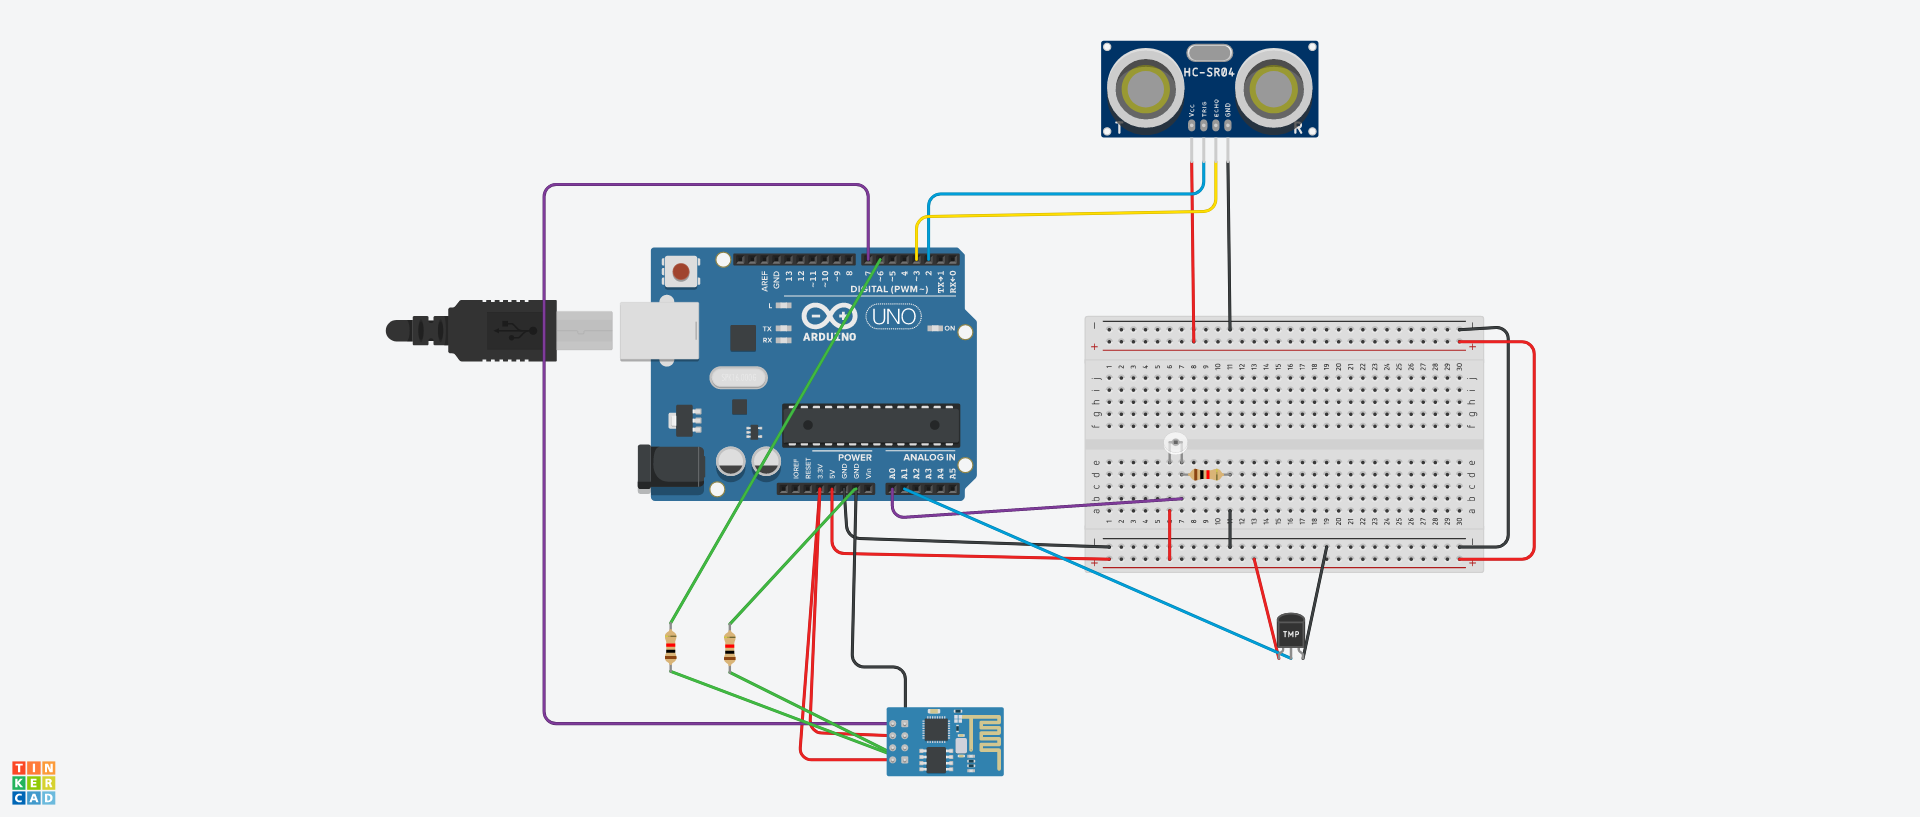
\includegraphics[scale=0.3]{scheme.png}
	\caption{Circuit that was built during the project}
	\label{fig:scheme}
\end{figure}

\section{User Interface}
\section{Google Cloud Mumpitz}

\end{document}